%% PNAStmpl.tex
%% Template file to use for PNAS articles prepared in LaTeX
%% Version: Apr 14, 2008


%%%%%%%%%%%%%%%%%%%%%%%%%%%%%%
%% BASIC CLASS FILE
%% PNAStwo for two column articles is called by default.
%% Uncomment PNASone for single column articles. One column class
%% and style files are available upon request from pnas@nas.edu.
%% (uncomment means get rid of the '%' in front of the command)

%\documentclass{pnasone}
\documentclass{pnastwo}

%%%%%%%%%%%%%%%%%%%%%%%%%%%%%%
%% Changing position of text on physical page:
%% Since not all printers position
%% the printed page in the same place on the physical page,
%% you can change the position yourself here, if you need to:

% \advance\voffset -.5in % Minus dimension will raise the printed page on the
                         %  physical page; positive dimension will lower it.

%% You may set the dimension to the size that you need.

%%%%%%%%%%%%%%%%%%%%%%%%%%%%%%
%% OPTIONAL GRAPHICS STYLE FILE

%% Requires graphics style file (graphicx.sty), used for inserting
%% .eps files into LaTeX articles.
%% Note that inclusion of .eps files is for your reference only;
%% when submitting to PNAS please submit figures separately.

%% Type into the square brackets the name of the driver program
%% that you are using. If you don't know, try dvips, which is the
%% most common PC driver, or textures for the Mac. These are the options:

% [dvips], [xdvi], [dvipdf], [dvipdfm], [dvipdfmx], [pdftex], [dvipsone],
% [dviwindo], [emtex], [dviwin], [pctexps], [pctexwin], [pctexhp], [pctex32],
% [truetex], [tcidvi], [vtex], [oztex], [textures], [xetex]

%\usepackage[dvips]{graphicx}

%%%%%%%%%%%%%%%%%%%%%%%%%%%%%%
%% OPTIONAL POSTSCRIPT FONT FILES

%% PostScript font files: You may need to edit the PNASoneF.sty
%% or PNAStwoF.sty file to make the font names match those on your system.
%% Alternatively, you can leave the font style file commands commented out
%% and typeset your article using the default Computer Modern
%% fonts (recommended). If accepted, your article will be typeset
%% at PNAS using PostScript fonts.

% Choose PNASoneF for one column; PNAStwoF for two column:
%\usepackage{PNASoneF}
\usepackage{PNAStwoF}

%%%%%%%%%%%%%%%%%%%%%%%%%%%%%%
%% ADDITIONAL OPTIONAL STYLE FILES

%% The AMS math files are commonly used to gain access to useful features
%% like extended math fonts and math commands.

\usepackage{amssymb,amsfonts,amsmath}

%\usepackage{subcaption}
\graphicspath{ {paper_figures2/} }

%\usepackage{sansmath}

%\usepackage[font={sf, small}]{caption}

%%%%%%%%%%%%%%%%%%%%%%%%%%%%%%
%% OPTIONAL MACRO FILES
%% Insert self-defined macros here.
%% \newcommand definitions are recommended; \def definitions are supported

%\newcommand{\mfrac}[2]{\frac{\displaystyle #1}{\displaystyle #2}}
%\def\s{\sigma}

\DeclareMathSizes{9}{8}{7}{7}

\DeclareMathOperator*{\argmin}{arg\,min}

\makeatletter
\newcommand{\customlabel}[2]{%
\protected@write \@auxout {}{\string \newlabel {#1}{{#2}{}}}}
\makeatother

%%%%%%%%%%%%%%%%%%%%%%%%%%%%%%
%% Don't type in anything in the following section:
%%%%%%%%%%%%
%% For PNAS Only:
\contributor{Submitted to Proceedings
of the National Academy of Sciences of the United States of America}
\url{www.pnas.org/cgi/doi/10.1073/pnas.0709640104}
\copyrightyear{2008}
\issuedate{Issue Date}
\volume{Volume}
\issuenumber{Issue Number}
%%%%%%%%%%%%

\begin{document}

%%%%%%%%%%%%%%%%%%%%%%%%%%%%%%


%% For titles, only capitalize the first letter
%% \title{Almost sharp fronts for the surface quasi-geostrophic equation}

\title{Temporal ordering and registration of cross-sectional imaging data}


%% Enter authors via the \author command.
%% Use \affil to define affiliations.
%% (Leave no spaces between author name and \affil command)

%% Note that the \thanks{} command has been disabled in favor of
%% a generic, reserved space for PNAS publication footnotes.

%% \author{<author name>
%% \affil{<number>}{<Institution>}} One number for each institution.
%% The same number should be used for authors that
%% are affiliated with the same institution, after the first time
%% only the number is needed, ie, \affil{number}{text}, \affil{number}{}
%% Then, before last author ...
%% \and
%% \author{<author name>
%% \affil{<number>}{}}

%% For example, assuming Garcia and Sonnery are both affiliated with
%% Universidad de Murcia:
%% \author{Roberta Graff\affil{1}{University of Cambridge, Cambridge,
%% United Kingdom},
%% Javier de Ruiz Garcia\affil{2}{Universidad de Murcia, Bioquimica y Biologia
%% Molecular, Murcia, Spain}, \and Franklin Sonnery\affil{2}{}}

\author{Carmeline~J.~Dsilva\affil{1}{Department of Chemical and Biological Engineering, Princeton University, Princeton, New Jersey, USA},
Bomyi~Lim\affil{1}{},
Thomas~J.~Levario\affil{2}{School of Chemical and Biomolecular Engineering, Georgia Institute of Technology, Atlanta, Georgia, USA},
Hang~Lu\affil{2}{},
Amit~Singer\affil{3}{Department of Mathematics, Princeton University, Princeton, New Jersey, USA} \affil{4}{Program in Applied and Computational Mathematics, Princeton University, Princeton, New Jersey, USA},
Stanislav~Y.~Shvartsman\affil{1}{} \affil{5}{Lewis-Sigler Institute for Integrative Genomics, Princeton University, Princeton, New Jersey, USA},
\and
Ioannis~G.~Kevrekidis\affil{1}{} \affil{4}{Program in Applied and Computational Mathematics, Princeton University, Princeton, New Jersey, USA}}

\contributor{Submitted to Proceedings of the National Academy of Sciences
of the United States of America}

%% The \maketitle command is necessary to build the title page.
\maketitle

%%%%%%%%%%%%%%%%%%%%%%%%%%%%%%%%%%%%%%%%%%%%%%%%%%%%%%%%%%%%%%%%
\begin{article}

\begin{abstract}
In studies of development, researchers are often presented with cross-sectional data, where each data point is a sample from a population fixed at a slightly different developmental time.
%
The goal is then to temporally order the data to reconstruct the developmental dynamics.
%
If each data point is a two-dimensional image, the images must first be registered before they can be temporally ordered.
%
When such data sets are large, noisy, and/or if the developmental changes are subtle, these tasks can be difficult to do by hand.
%
We present an automatic approach to register {\it and} temporally order cross-sectional data sets of images.
%
The mathematical techniques (vector diffusion maps) are applicable to a wide variety of data sets and
require little {\it a priori} knowledge of the image features or the developmental dynamics.
%
We demonstrate the utility of our methods using a collection of images from a study of {\it Drosophila} embryogenesis.
\end{abstract}


%% When adding keywords, separate each term with a straight line: |
\keywords{temporal ordering | image registration}

%% Optional for entering abbreviations, separate the abbreviation from
%% its definition with a comma, separate each pair with a semicolon:
%% for example:
%% \abbreviations{SAM, self-assembled monolayer; OTS,
%% octadecyltrichlorosilane}

% \abbreviations{}

%% The first letter of the article should be drop cap: \dropcap{}
%\dropcap{I}n this article we study the evolution of ''almost-sharp'' fronts

%% Enter the text of your article beginning here and ending before
%% \begin{acknowledgements}
%% Section head commands for your reference:
%% \section{}
%% \subsection{}
%% \subsubsection{}



\dropcap{E}xperimental studies of developmental dynamics fall in two broadly defined categories: longitudinal and cross-sectional \cite{diggle2002analysis}.
%
In longitudinal studies, developmental progress is monitored over time for the same embryo.
%
In a cross-sectional study, one embryo contributes only a single snapshot of a chemical or morphological process along its developmental trajectory, and the developmental dynamics must be reconstructed from multiple snapshots of different embryos.
%
Both of these sampling schemes have their advantages and limitations, and both are extensively used by developmental biologists.
%
Here we focus on cross-sectional studies, which have a time-honored history and still present the only option for most organisms.
%
In a typical cross-sectional study, a group of developing embryos is fixed using a procedure that arrests their development and stained with chemicals that help visualize a handful of cellular processes.
%
Fixed embryos are then imaged using any given number of microscopy techniques.
%
Recent advances in large-scale physical manipulation and imaging of embryos have produced rapidly increasing volumes of cross-sectional data, in which every embryo is observed at a different geometric orientation and developmental time point.
%
Importantly, the ``age'' of any given embryo arrested in its development is not known to high accuracy.
%
In general, it is only known that a collection of embryos belongs to a certain time window.
%
In order to recover the developmental dynamics from such image datasets, snapshots of different embryos must be spatially aligned or registered to factor out the relevant symmetries (i.e., translations and rotations), and then ordered in time.
%
We show how existing dimensionality reduction algorithms can greatly accelerate -and combine- both of these tasks.

Temporal ordering and registration of images is straightforward when the number of images is small and differences between them are visually apparent.
%
As an example, Figure~\ref{fig:fish} shows a caricature of fish development, combining the processes of growth and color patterning.
%
In this case, temporal ordering can be accomplished by arranging the fish by size, which is monotonic with the developmental progress.
%
Image registration is based on obvious morphological landmarks, such as the position of head and fins.
%
On the other hand, real data poses nontrivial challenges, due to the number of images, measurement noise and variability, and the subtlety of the developmental changes.

\begin{figure}[t]
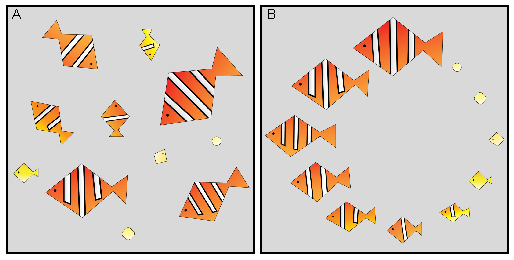
\includegraphics[width=8.4cm]{fig1}
\caption{{\it (A)} Fish, each in a different orientation and a different stage of development. {\it (B)} Fish, now rotationally registered and temporally ordered. For this caricature, the registration and ordering is easy to do ``by hand" because the data set is small and the developmental changes are easy to recognize.}
%\label{fig:fish}
\customlabel{fig:fish}{1}
\customlabel{subfig:fish_unordered}{\ref{fig:fish}{\it A}}
\customlabel{subfig:fish_ordered}{\ref{fig:fish}{\it B}}
\end{figure}

We will show that we can use existing dimensionality reduction techniques to register and temporally order large sets of images from developmental biology studies. 
%
We will demonstrate these techniques using two data sets from a study of {\it Dropophila} embryogenesis.
%
The first data set, shown in Figure~\ref{subfig:raw_data1}, is relatively simple and will allow us to both illustrate and validate our methods. 
%
In the second data set, shown in Figure~\ref{subfig:raw_data2}, the dynamics are significantly more complex; here, we will show that we can recover a reasonable trajectory that is qualitatively consistent with current knowledge.

In both of these data sets, each image is taken from a different embryo, fixed at a different developmental time and imaged in a different rotational orientation.
%
We would like to organize these data sets in a meaningful and informative way.
%
This requires rotating and translating each image so the set is in a consistent frame of reference ({\it registration}), and then temporally ordering the images. 
%
We will show that dimensionality reduction algorithms can accomplish both of these tasks and therefore give us a meaningful picture of the underlying developmental dynamics. 


\begin{itemize}
\item Imaging data is becoming increasingly prevalent in biology research.
%
\item General motivation about biology data ...
%
\item Need methods to organize data, visualize, ...
%
\item REDUCTION is important, reduction because of symmetry and reduction because of content
%
\item There are a bunch of recent techniques- some established (like dmaps), some very fresh, like synchronization or VDMaps,  that have had their own reasons to be developed but they are as if tailor made for what we would want to do
\end{itemize}


\section{Results and Discussion}

%Rank corr for data set 1 using VDM=  0.9127

%Variance captured by PC 1 for data set 2 = 0.2155

\subsection{Vector diffusion maps for registration and temporal ordering}

We use vector diffusion maps \cite{singer2012vector} to automatically register and order our images.
%
Vector diffusion maps is a general technique, developed for data sets which contain both symmetries (e.g., translations and rotations) which one would like to factor out, and other directions of variability which one would like to uncover.
%
It combines two algorithms, angular synchronization \cite{singer2011angular} for registration and diffusion maps \cite{coifman2005geometric} for extracting low-dimensional structure, into one computation that allows us to simultaneously register and temporally order our images. 
%
Vector diffusion maps has been applied to cryo-EM images \cite{...}, where each image is a (very noisy) projection of a molecule, taken from a different viewing direction and in a different rotation. 
%
Here, we will use it to register the images with respect to rotations and translations, as well as uncover the main direction of variability, which is parameterized by time. 
%
The noise in our experiments is primarily from interembryo variability, rather than white noise from a measurement instrument (as in the cryo-EM example). 

Registration via angular synchronization/vector diffusion maps uses pairwise alignment information to globally register the images in a consistent way.
%
A schematic illustration is shown in Figure~\ref{subfig:synchron1}; each image is depicted as a vector, and the goal is to align the set of vectors. 
%
We first compute the angles needed to align pairs of vectors (or images).
%
This is rather simple to do, and requires no template function; however, when the images are noisy, some pairwise alignment angles may be inaccurate.
%
Using the angles between all pairs of vectors (or images), angular synchronization/vector diffusion maps then finds the set of rotation angles, one angle for each vector, that is most consistent with the pairwise measurements.

In general, diffusion maps \cite{coifman2005geometric} is a nonlinear dimensionality reduction technique;
it uncovers a parameterization of data that lies on a low-dimensional (perhaps nonlinear) manifold in high-dimensional space. 
%
This idea is illustrated in Figure~\ref{subfig:dmaps1}: the data are two-dimensional points which lie on a one-dimensional nonlinear curve. 
%
The color in Figure~\ref{subfig:dmaps2} depicts the one-dimensional parameterization or ordering of the data that we can detect visually.
%
In our examples, each data point will be very high dimensional (e.g, an image with many pixels), and so we cannot extract this low-dimensional structure visually.
%
Instead, we will rely on diffusion maps to automatically extract a parameterization of our high-dimensional data.
%
We will assume that our data are (approximately) one-dimensional, and that this dimension is parameterized by time.
%
Therefore, ordering our data along this main dimension/direction will temporally order our data. 
%
Vector diffusion maps combines angular synchronization and diffusion maps to find a parameterization of the data while simultaneously registering data points which are close.

\begin{figure}[t]
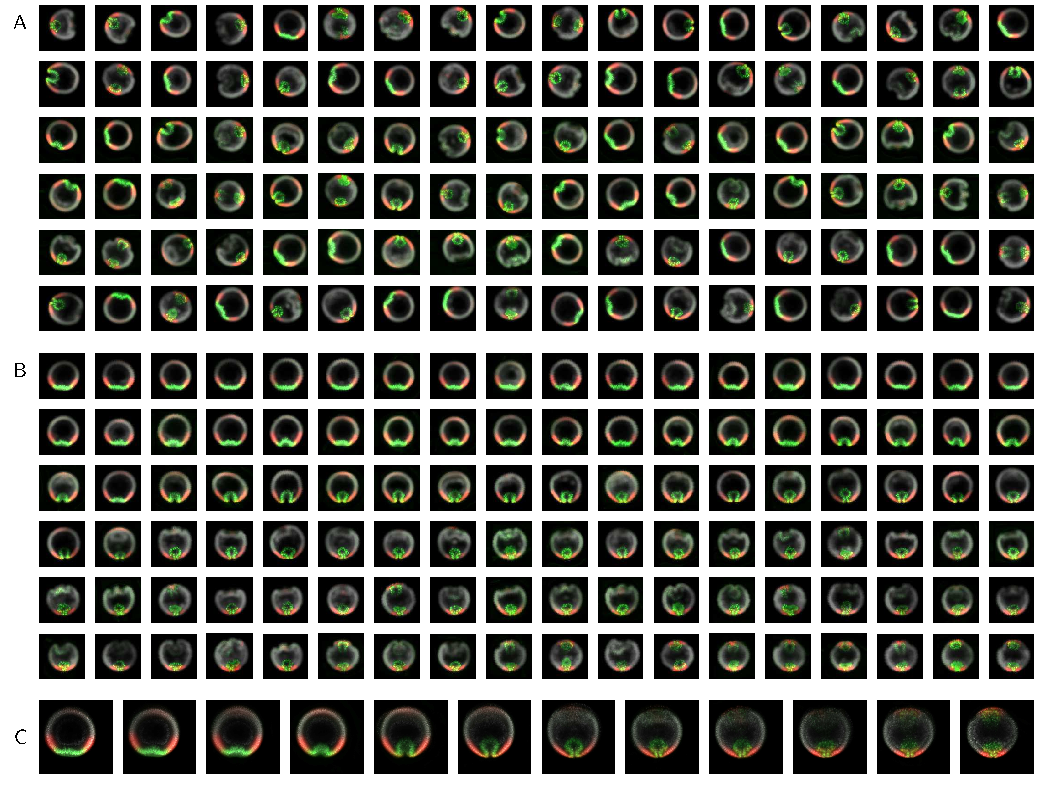
\includegraphics[width=8.4cm]{fig4}
\caption{ {\it (A)} Set of vectors, each in a different orientation. The pairwise alignment angles are indicated. {\it (B)} The vectors from {\it A}, each rotated so that the set is globally aligned. Note that the chosen rotation angles are consistent with the pairwise alignments in {\it A}. {\it (C)} Data points (in black) which lie on a one-dimensional nonlinear curve in two dimensions. Each pair of data points is connected by an edge, and the edge weight is related to the Euclidean distance between the points through the diffusion kernel (see {\it SI Appendix}), so that close data points are connected by dark (``stronger'') edges. {\it (D)} The data in {\it C}, colored by the first (non-trivial) eigenvector from the diffusion map computational procedure, $\phi_2$. The color intensity is monotonic with the arclength, thus parameterizing the curve.}
%\label{fig:schematics}
\customlabel{fig:schematics}{2}
\customlabel{subfig:synch1}{\ref{fig:schematics}{\it A}}
\customlabel{subfig:synch2}{\ref{fig:schematics}{\it B}}
\customlabel{subfig:dmaps1}{\ref{fig:schematics}{\it C}}
\customlabel{subfig:dmaps2}{\ref{fig:schematics}{\it D}}
\end{figure}


\subsection{Stage 5 images in {\it Drosophila} embryogenesis}

Our first data set, shown in Figure~\ref{subfig:raw_data1}, consists of $49$ images from stage 5 of {\em Drosophila} embryogenesis.
%
Each image is from a different embryo imaged in a different orientation and fixed at a different developmental time. 
%
We registered and ordered the images using vector diffusion maps.
%
The results are shown in Figure~\ref{subfig:ordered_data1}.
%
The features that our eyes can visually detect (the green Dorsal peak, and the red dpERK peaks) are now consistently registered, even though the algorithm does not require any information about the existence or location of these peaks. 

When dealing with large sets of images with interembryo variability, we can gain a better understanding of the developmental dynamics by looking at an averaged trajectory.
%
Figure~\ref{subfig:average_data1} shows the moving average of the trajectory in Figure~\ref{subfig:ordered_data1}. 
%
We can now easily see the developmental dynamics: the red dpERK peaks grow in time, and the ventral furrow (the dent in green) begins to form at the end of stage 5. 

For this data set, we can validate our proposed vector diffusion maps ordering of the data.
%
During stage 5, we can measure the developmental time of each embryo based on the monotonic progress of cellularization (details are given in the {\it SI Appendix}).
%
We compared the temporal ordering obtained from cellularization with the ordering we extract from vector diffusion maps. 
%
The rank correlation coefficient between these two orderings is 0.9127, indicating that there is very good agreement and vector diffusion maps is uncovering the correct temporal ordering of the images. 

\begin{figure*}[t]
\raisebox{8.1cm}{{\figtextfont A}}
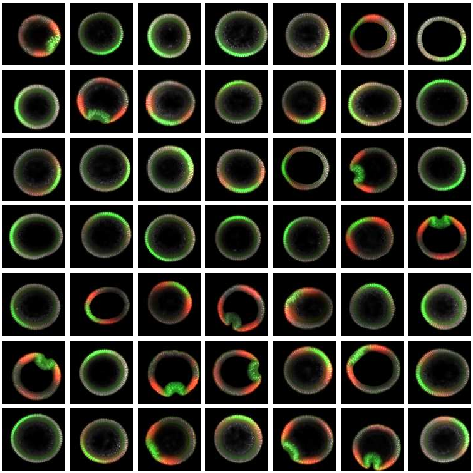
\includegraphics[width=8.4cm]{raw_data1}
\hfill
\raisebox{8.1cm}{{\figtextfont B}}
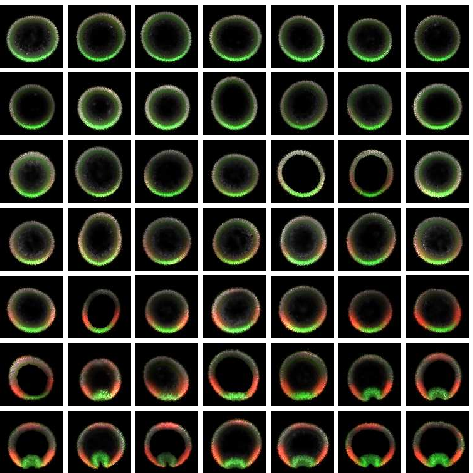
\includegraphics[width=8.4cm]{VDM_data1_ordered}\\
\vspace{0.2cm}
\centering
\raisebox{0.5cm}{{\figtextfont C}}
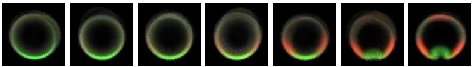
\includegraphics[width=8.4cm]{average_trajectory_VDM}
\caption{{\it (A)} Images from stage 5 of {\it Drosophila} embryogenesis. Each image is of a different embryo in a different rotational orientation. {\it (B)} Images from {\it A}, now registered and ordered using vector diffusion maps. {\it (C)} Average trajectory of the images shown in {\it B}.  Each image is the average of $7$ consecutive images in {\it B}. }
\customlabel{fig:data1}{3}
\customlabel{subfig:raw_data1}{\ref{fig:data1}{\it A}}
\customlabel{subfig:ordered_data1}{\ref{fig:data1}{\it B}}
\customlabel{subfig:averaged_data1}{\ref{fig:data1}{\it C}}
\end{figure*}


\subsection{Stage 5--7 Images of {\it Drosophila} embryogenesis}

The images in Figure~\ref{fig:data1} are relatively simple, and the methods presented here are perhaps unnecessarily complex for this particular data set. 
%
Because these data are effectively a single mode growing in time,
principal component analysis \cite{shlens2005tutorial} would uncover most of the meaningful structure in the data, and projection onto the first principal component would be sufficient to order the data.
%
However, developmental dynamics are often significantly more complex, and nonlinear techniques such as diffusion maps/vector diffusion maps are required to extract meaningful structure in the data. 
%
Figure~\ref{subfig:raw_data2} shows a data set of $108$ images from stages 5--7 of {\it Drosophila} embryogenesis.
%
Only 22\% of the variability in the data is captured by the first principal component, and so we are forced to use more sophisticated techniques, such as vector diffusion maps, to temporally order the data.

Figure~\ref{subfig:ordered_data2} shows the images in Figure~\ref{subfig:raw_data2}, now registered and ordered using vector diffusion maps \cite{singer2012vector}.
%
Again, visually detectable features, such as the green Twist peaks, are consistently aligned. 
%
Unlike the images in Figure~\ref{subfig:raw_data1}, 
for Figure~\ref{fig:data2}, we have no time marker with which to validate our orderings.
%
However, there are noticeable features in the ordering that we can see are consistent with previously known dynamics.
%
We can again construct a smoothed trajectory by looking at the moving average of the images, shown in Figure~\ref{subfig:averaged_data2}.
%
We can see the formation of the ventral furrow and germ band elongation, which concludes with ventral cells shifted to the dorsal side of the embryo, which is consistent with the known picture of {\it Drosophila} embryogeneisis. 
%
This assures us that we can obtained an ordering of the data which is developmentally meaningful. 

\newpage
\begin{figure*}[t]
\raisebox{5.3cm}{{\figtextfont A}}
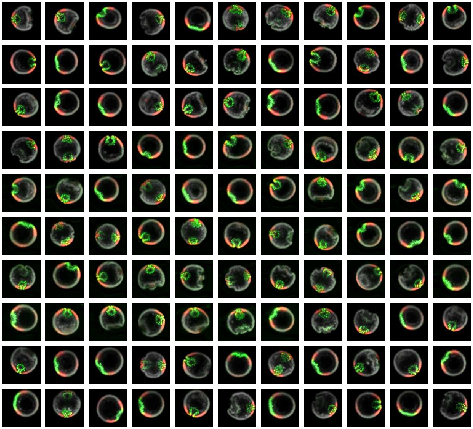
\includegraphics[width=16.8cm]{raw_data2}

\vspace{0.2cm}
\raisebox{5.3cm}{{\figtextfont B}}
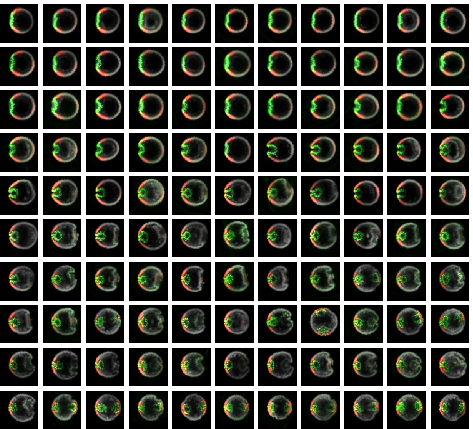
\includegraphics[width=16.8cm]{VDM_ordered}

\vspace{0.2cm}
\raisebox{0.6cm}{{\figtextfont C}}
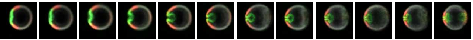
\includegraphics[width=16.8cm]{average_trajectory}
\caption{{\it (A)} Images from stages 5-7 of {\it Drosophila} embryogenesis. Each image is of a different embryo in a different rotational orientation. {\it(B)} Data from {\it A}, registered and ordered using vector diffusion maps. {\it (C)} Average trajectory of the images shown in {\it B}. Each image is the average of $9$ consecutive images in {\it B}. }
\customlabel{fig:data2}{4}
\customlabel{subfig:raw_data2}{\ref{fig:data2}{\it A}}
\customlabel{subfig:ordered_data2}{\ref{fig:data2}{\it B}}
\customlabel{subfig:averaged_data2}{\ref{fig:data2}{\it C}}
\end{figure*}

\section{Conclusions}

We have demonstrated how existing reduction techniques (vector diffusion maps) can be used to register and temporally order images from developmental biology studies. 
%
We acknowledge that the tasks of both registration and ordering can be accomplished using a variety of techniques.
%
We chose the techniques outlined here, not because they are particularly suited to this specific problem, but rather, because they are sufficiently general and we are confident that they can be applied to a myriad of biological imaging applications. 

The task of image registration has been studied in a variety of contexts \cite{...}.
%
However, most of these applications rely on the definition and identification of good {\it features} within each image. 
%
For our biological applications, good features may not be known {\it a priori}, 
and we instead use an algorithm which requires no features, but instead, uses the images directly. 

The task of temporal ordering has also been studied, for data such as ...
%
Most of these applications order the data by solving a traveling salesman problem or constructing a minimum spanning tree on the data,
expecting that these structures (the path of the traveling salesman, or the minimum spanning tree) characterize the majority of the structure/variability within the data and provide an accurate encoding of the dynamical progression.
%
We, instead, use diffusion maps to construct a one-dimensional parameterization of the data.
%
Diffusion maps are one of many nonlinear dimensionality reduction techniques that have been recently developed \cite{Belkin2003, tenenbaum2000global, Donoho2003, Roweis2000}.
%
They have been shown to be more robust to noise than other path-based algorithms, such as isomap \cite{balasubramanian2002isomap}, and so we suspect they may perform better than the ordering algorithms used in previous work.
% 
Furthermore, techniques such as diffusion maps do not constrain us to one-dimensional parameterizations/organizations of the data.
% 
In this particular setup, we expect our data to be one-dimensional, as the only (main) source of variability is time.
%
However, other sources of variability would also be uncovered using (vector) diffusion maps, 
and tasks such as classification of embryos by size or viewing angle, and comparison of different mutations can also be accomplished using the same techniques. 


\begin{itemize}
\item What are other people doing  (maybe critically)
\item Movies  smoothness
\item Discrete symmetries like flips
\item Local information ? (features of the image) (associate with Fourier-Bessel and bispectra)
\item Mutant-wildtype stuff  IMPORTANT
\item And in general, MULTIPLE variablities is important (mutants, guys in another cycle, etc.)
 
\item size is an issue
\item  small tilts is an issue
\item   could one do three-d image processing ?  of the floating thing, without the device
\item how do we go about merging datasets ?
\end{itemize}



\bibliographystyle{pnas}
\bibliography{background_reading/references,../../references/references}

\end{article}

\end{document}

